


\begin{figure}[htb]
\centering
\includegraphics[page=6,width=0.45\textwidth]{\FCNCFigures/xTFW/raw/NOMINAL/reg2mtau1b2jss/tau_pt_0.pdf}
\put(-100, 140){\textbf{(a)}}
\put(-120, 130){\footnotesize{STH $\thadhad$ (SS)}}
\includegraphics[page=6,width=0.45\textwidth]{\FCNCFigures/xTFW/raw/NOMINAL/reg2mtau1b2jos/tau_pt_0.pdf}
\put(-100, 140){\textbf{(b)}}
\put(-120, 130){\footnotesize{STH $\thadhad$ (OS)}}\\
\includegraphics[page=6,width=0.45\textwidth]{\FCNCFigures/xTFW/raw/NOMINAL/reg2mtau1b3jss/tau_pt_0.pdf}
\put(-100, 140){\textbf{(c)}}
\put(-120, 130){\footnotesize{TTH $\thadhad$ (SS)}}
\includegraphics[page=6,width=0.45\textwidth]{\FCNCFigures/xTFW/raw/NOMINAL/reg2mtau1b3jos/tau_pt_0.pdf}
\put(-100, 140){\textbf{(d)}}
\put(-120, 130){\footnotesize{TTH $\thadhad$ (OS)}}
\caption{ The distributions of $\tau$ $\pt$ in the STH $\thadhad$ (SS)(a), STH $\thadhad$ (OS) (b), TTH $\thadhad$ (SS) (c) 
and TTH $\thadhad$ (OS) (d), to illustrate the background composition. Data is more than the prediction because the fake tau backgrounds are missing. }
\label{fig:os_pre_hadhad}
\end{figure}

